\documentclass{article}
\linespread{1.3}
\usepackage[margin=50pt]{geometry}
\usepackage{amsmath, amsthm, amssymb, amsthm, tikz, fancyhdr, graphicx, subfig}
\pagestyle{fancy}
\renewcommand{\headrulewidth}{0pt}
\newcommand{\changefont}{\fontsize{15}{15}\selectfont}

\newcommand{\field}[1]{\mathbb{#1}}
\newcommand{\1}{\mathbf{1}}
\newcommand{\E}{\mathbb{E}} 
\renewcommand{\P}{\mathbb{P}}
\newcommand{\R}{\field{R}} % real domain
% \newcommand{\C}{\field{C}} % complex domain
\newcommand{\F}{\field{F}} % functional domain

\newcommand{\T}{^{\textrm T}} % transpose

\def\diag{\text{diag}}

%% operator in linear algebra, functional analysis
\newcommand{\inner}[2]{#1\cdot #2}
\newcommand{\norm}[1]{\left\|#1\right\|}
\newcommand{\twonorm}[1]{\|#1\|_2^2}
% operator in functios, maps such as M: domain1 --> domain 2
\newcommand{\Map}[1]{\mathcal{#1}}
\renewcommand{\theenumi}{\alph{enumi}} 

\newcommand{\Perp}{\perp \! \! \! \perp}

\newcommand\independent{\protect\mathpalette{\protect\independenT}{\perp}}
\def\independenT#1#2{\mathrel{\rlap{$#1#2$}\mkern2mu{#1#2}}}
\newcommand{\vct}[1]{\boldsymbol{#1}} % vector
\newcommand{\mat}[1]{\boldsymbol{#1}} % matrix
\newcommand{\cst}[1]{\mathsf{#1}} % constant
\newcommand{\ProbOpr}[1]{\mathbb{#1}}
\newcommand{\points}[1]{\small\textcolor{magenta}{\emph{[#1 points]}} \normalsize}
\date{{}}

\fancypagestyle{firstpageheader}
{
  \fancyhead[R]{\changefont Michael Huang \\ CSE 446 \\ Homework 3}
}

\begin{document}

\thispagestyle{firstpageheader}

\section*{Collaborators}
{\Large 
Jimmy Guo, Neil Kagalwala, Andrew Wang
}
\section*{A.1}
{\Large 

\subsection*{a.}

If the RBF kernel underfits the training set, we should decrease the bandwidth $\sigma$. Underfitting indicates a smoother fit and lower variance, so we want to decrease $\sigma$ so that we fit the training points more tightly.
% more narrow bumps and fits data more tightly

\subsection*{b.}

True. With a non-convex loss function, gradient descent is not guaranteed to go all the way towards the global minimum, and could even stagnate or increase.
% Could increase?

\subsection*{c.}

False. When training a deep neural network, we should initialize weights to random values. One reason for this is that with any equal weight initialization, all nodes will have the same gradient, so the nodes will end up all following the same pattern and an ineffective model overall.

\subsection*{d.}

True. We try to use non-linear activation functions in order to introduce non-linearity into the network. If we only had linear activation functions, then the model would essentially just output a linear function, since no matter how many layers, all the linear functions would naturally sum together, and lead to what is essentially basic logistic regression.

\subsection*{e.}

True. The time complexity for the forward pass is lower than that of the backward pass in the backpropagation algorithm. backpropagation first requires calculating values via forward-propagation itself, and then performing error calculation and gradient descent to update these values.

}

\section*{A.2}
{\Large

We aim to show that $K(x, x') = e^{-\frac{(x-x')^2}{2}}$ is a kernel function for the defined feature map, or that $\phi (x) \cdot \phi (x') = e^{-\frac{(x-x')^2}{2}}$. \\ \\
We are given that the $i$th component of the vector $\phi(x)$ is defined as $\frac{1}{\sqrt{i!}} e^{-x^2/2} x^i$, and we can naturally express $\phi(x')$ as  $\frac{1}{\sqrt{i!}} e^{-(x')^2 / 2} (x')^i$.
% $= \sqrt{\frac{e^{-x^2}}{i}} x^i$
\\
In multiplying $\phi(x) \cdot \phi(x')$, we have that we are essentially multiplying the elements of each column against each other, that is, $\phi(x) \cdot \phi(x')$ \\
$= \sum_{i=0}^{n} \text{element}_i \text{ of } \phi(x) \cdot \text{element}_i \text{ of } \phi(x')$ \\
$= \sum_{i=0}^{n} \frac{1}{\sqrt{i!}} e^{-x^2/2} x^i \cdot \frac{1}{\sqrt{i!}} e^{-(x')^2 / 2} (x')^i$ \\
$= \sum_{i=0}^{n} \frac{1}{i!} e^{-x^2/2} x^i \cdot e^{-(x')^2 / 2} (x')^i$ \\
$= \sum_{i=0}^{n} \frac{1}{i!} e^{-x^2/2 - (x')^2 / 2} x^i (x')^i$ \\
$= e^{-x^2/2 - (x')^2 / 2} \cdot \sum_{i=0}^{n} \frac{1}{i!} (xx')^i$ \\ \\
% maybe change the n to \infty
We know that the Taylor series expansion of $z \mapsto e^z$ is $\sum_{i=0}^{\infty} \frac{z^i}{i!}$ to simplify the second term of the product, as we know that $\phi(x)$ is a vector of infinite length: \\
$= e^{-x^2/2 - (x')^2 / 2} \cdot e^{(xx')}$ \\
$= e^{-x^2/2 - (x')^2 / 2 + (xx')} $ \\
$= e^{\frac{-x^2 - (x')^2 + 2xx'}{2}} $ \\
$= e^{\frac{-(x^2 + (x')^2 - 2xx')}{2}} $ \\
$= e^{\frac{-(x - x')^2)}{2}} $ \\
which is exactly what we sought to show.

}

\newpage
\section*{A.3}

{\Large 

\subsection*{a.}

\textbf{poly:} \\
$d: 18.0$ \\
$\lambda: 10^{-5}$ \\ 
\textbf{rbf:} \\
$\gamma: 30$ \\
$\lambda: 10^{-1}$

\subsection*{b.}

\begin{figure}[h]
  \centering
  \subfloat[poly true vs predict]{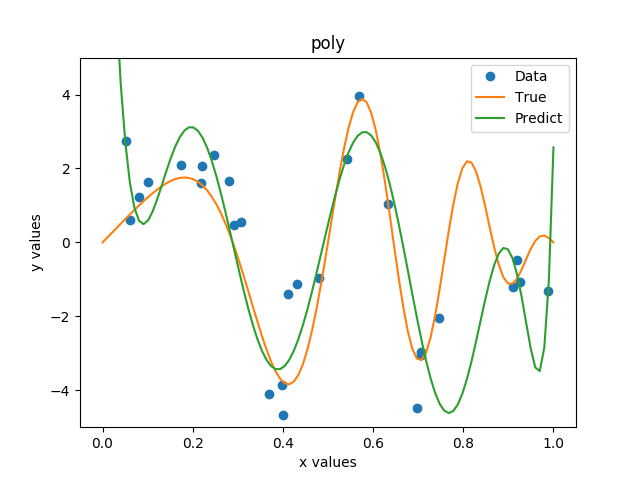
\includegraphics[width=100mm]{../hw3-code/results/a3_bi.png}}
  \subfloat[rbf true vs predict]{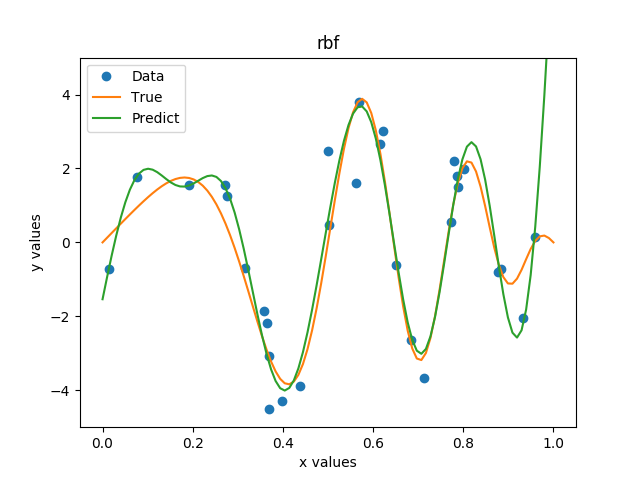
\includegraphics[width=100mm]{../hw3-code/results/a3_bii.png}}
\end{figure}

\newpage

\subsection*{c.}

\begin{figure}[h]
  \centering
  \subfloat[poly with confidence intervals]{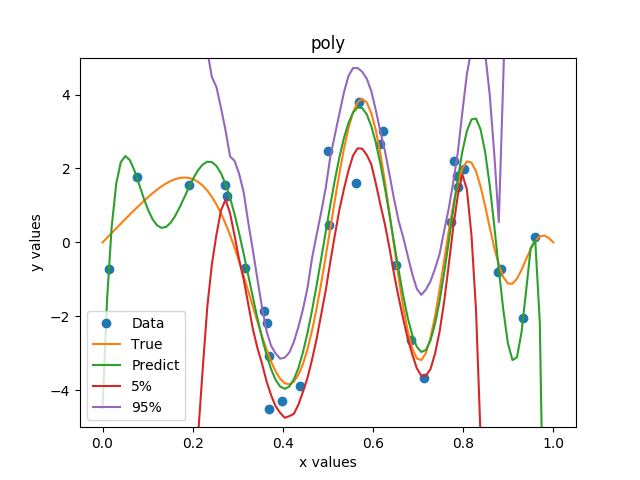
\includegraphics[width=100mm]{../hw3-code/results/a3_ci.png}}
  \subfloat[rbf with confidence intervals]{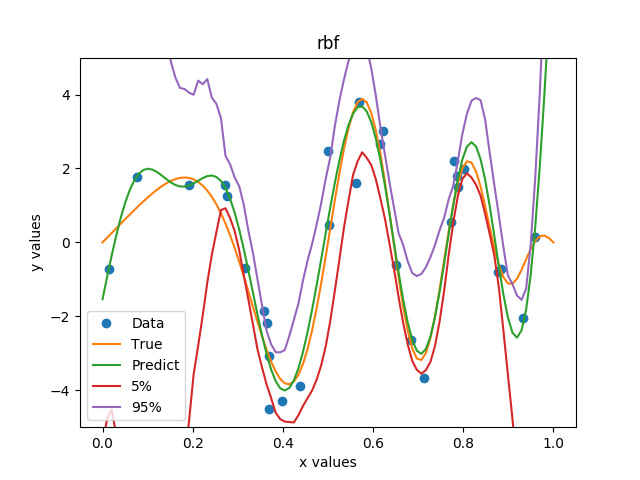
\includegraphics[width=100mm]{../hw3-code/results/a3_cii.png}}
\end{figure}

\subsection*{d.}
\begin{figure}[h]
  \centering
  \subfloat[poly true vs predict]{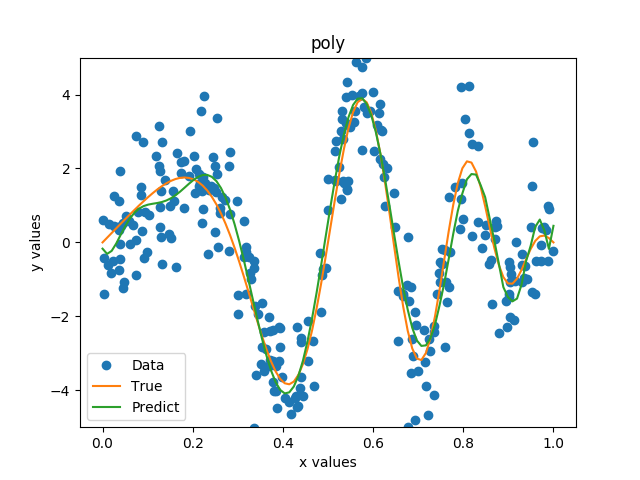
\includegraphics[width=100mm]{../hw3-code/results/a3_d.bi.png}}
  \subfloat[rbf true vs predict]{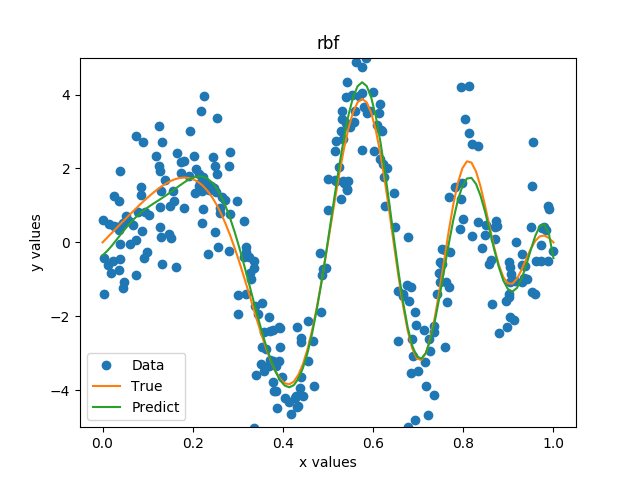
\includegraphics[width=100mm]{../hw3-code/results/a3_d.bii.png}}
\end{figure}
\begin{figure}[h]
  \centering
  \subfloat[poly with confidence intervals]{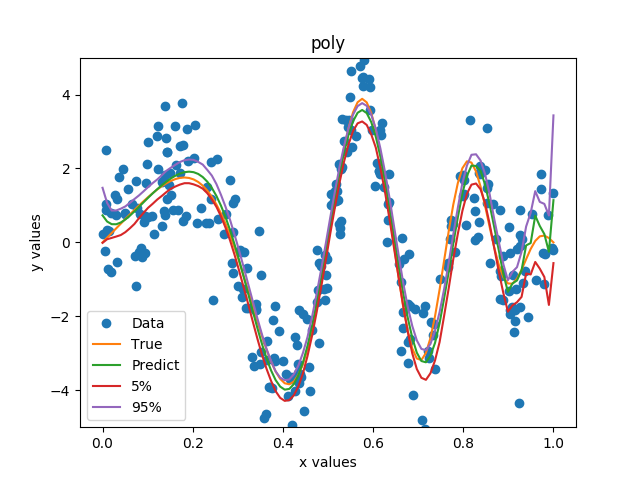
\includegraphics[width=100mm]{../hw3-code/results/a3_d.ci.png}}
  \subfloat[rbf with confidence intervals]{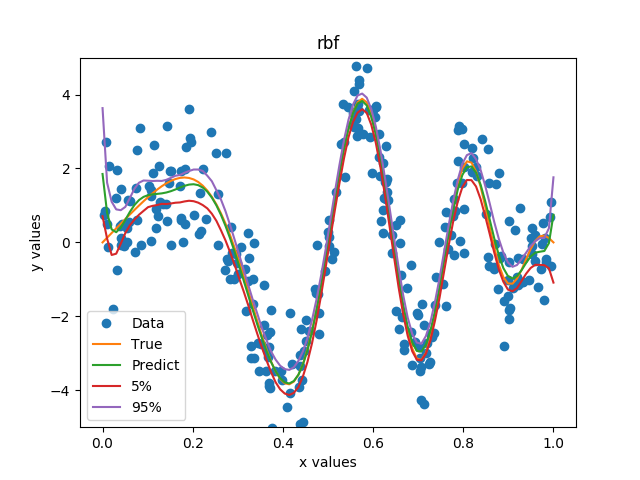
\includegraphics[width=100mm]{../hw3-code/results/a3_d.cii.png}}
\end{figure} 
\newpage
\textbf{poly:} \\
$d: 22.0$ \\
$\lambda: 10^{-7}$ \\ 
\textbf{rbf:} \\
$\gamma: 24.0$ \\
$\lambda: 10^{-4}$

\subsection*{e.}

5\%: 0.33408841623035646 \\
95\%: 0.6405912247916652 \\
Using this confidence interval, which is all positive and does not include 0, there does appear to be statistically significant evidence to suggest that one is the better. Since the way the estimator is constructed has the differences in actual vs predicted values for the polynomial kernel subtracted by that of the rbf kernel, we can see that the differences are greater in the polynomial kernel, which tells us that the rbf kernel seems to be a better predictor in a statistically significant manner.

\begin{verbatim}
# kernel.py
# Applicable code for HW3 A3

import numpy as np

import constants as c
import helpers as h

to_run = {
  "abc" : True,
  "de" : True,
}

def main():

  X, Y, true_f = h.generate_data(30)

  # individual elements over entire matrix
  kf_poly = lambda x, z, d: (1 + x * z) ** d
  kf_rbf = lambda x, z, gamma: np.exp(-gamma * ((x - z) ** 2))

  if to_run["abc"]:
    """
    part (a)
    """

    k_poly = Kernel(X, Y, kf_poly)
    k_rbf = Kernel(X, Y, kf_rbf)

    """
    part (b)
    """

    true_data = [true_f(x_val) for x_val in c.x_list]
    poly_pred_data = k_poly.get_fhat_data(X, Y)
    rbf_pred_data = k_rbf.get_fhat_data(X, Y)

    poly_list = [true_data, poly_pred_data]
    rbf_list = [true_data, rbf_pred_data]

    h.plot_multiple("poly", "a3_bi", X, Y, poly_list, c.pred_labels, c.a3b_ylimits)
    h.plot_multiple("rbf", "a3_bii", X, Y, rbf_list, c.pred_labels, c.a3b_ylimits)

    """
    part (c)
    """

    poly_5, poly_95 = k_poly.bootstrap(c.B)
    rbf_5, rbf_95 = k_rbf.bootstrap(c.B)

    poly_list = [true_data, poly_pred_data, poly_5, poly_95]
    rbf_list = [true_data, rbf_pred_data, rbf_5, rbf_95]

    h.plot_multiple("poly", "a3_ci", X, Y, poly_list, c.pct_labels, c.a3b_ylimits)
    h.plot_multiple("rbf", "a3_cii", X, Y, rbf_list, c.pct_labels, c.a3b_ylimits)

  if to_run["de"]:

    """
    part (d)
    """

    # repeated a
    X, Y, true_f = h.generate_data(300)

    k_poly = Kernel(X, Y, kf_poly, kfold=True)
    k_rbf = Kernel(X, Y, kf_rbf, kfold=True)

    # repeated b
    true_data = [true_f(x_val) for x_val in c.x_list]
    poly_pred_data = k_poly.get_fhat_data(X, Y)
    rbf_pred_data = k_rbf.get_fhat_data(X, Y)

    poly_list = [true_data, poly_pred_data]
    rbf_list = [true_data, rbf_pred_data]

    h.plot_multiple("poly", "a3_d.bi", X, Y, poly_list, c.pred_labels, c.a3b_ylimits)
    h.plot_multiple("rbf", "a3_d.bii", X, Y, rbf_list, c.pred_labels, c.a3b_ylimits)

    # repeated c
    poly_5, poly_95 = k_poly.bootstrap(c.B)
    rbf_5, rbf_95 = k_rbf.bootstrap(c.B)

    poly_list = [true_data, poly_pred_data, poly_5, poly_95]
    rbf_list = [true_data, rbf_pred_data, rbf_5, rbf_95]

    h.plot_multiple("poly", "a3_d.ci", X, Y, poly_list, c.pct_labels, c.a3b_ylimits)
    h.plot_multiple("rbf", "a3_d.cii", X, Y, rbf_list, c.pct_labels, c.a3b_ylimits)

    """
    part (e)
    """

    X, Y, true_f = h.generate_data(c.m)

    poly_pred = k_poly.kernel_rr(X, Y, k_poly.hp, k_poly.lamb)
    rbf_pred = k_rbf.kernel_rr(X, Y, k_rbf.hp, k_rbf.lamb)

    bs_5, bs_95 = get_bootstrap_values(X, Y, poly_pred, rbf_pred)

    print(bs_5)
    print(bs_95)

def get_bootstrap_values(X, Y, poly_pred, rbf_pred, m=c.m, B=c.B):
  
  diff_list = np.zeros(B)

  for i in range(B):
    
    index_samples = np.random.choice(m, m)

    x_b = X[index_samples]
    y_b = Y[index_samples]

    poly_diff = (np.abs(y_b - [poly_pred(x) for x in x_b]) ** 2)
    rbf_diff = (np.abs(y_b - [rbf_pred(x) for x in x_b]) ** 2)

    diff_list[i] = (1 / m) * np.sum(poly_diff - rbf_diff)


  bs_5 = np.percentile(diff_list, 5, axis=0)
  bs_95 = np.percentile(diff_list, 95, axis=0)

  return bs_5, bs_95

class Kernel:
  def __init__(self, X, Y, kernel_func=None, hyperparameter=None, lambda_reg=None, kfold=False):
    self.X = X
    self.Y = Y
    self.kf = kernel_func
    self.hp = hyperparameter
    self.lamb = lambda_reg
    self.kmat = None

    if self.hp is None and self.lamb is None:
      print("setting best hyperparameter, lambda")

      if kfold:
        self.kfold_cv()
      else:
        self.loo_cv()
      

    print("hyperparam: " + str(self.hp))
    print("lambda: " + str(self.lamb))

  def get_fhat_data(self, x, y):
    pred_f = self.kernel_rr(x, y, self.hp, self.lamb)

    return [pred_f(x_val) for x_val in c.x_list]

  def loo_cv(self):
    n = len(self.X)

    error_matrix = np.zeros((len(c.hp_list), len(c.lamb_list)))

    # try every combo and keep track of errors
    for i, hp in enumerate(c.hp_list):
      for j, lamb in enumerate(c.lamb_list):
        for k in range(n):
          X_val = self.X[k]
          Y_val = self.Y[k]
          
          # train without the loo val
          X_train = np.concatenate((self.X[:k], self.X[k + 1:]))
          Y_train = np.concatenate((self.Y[:k], self.Y[k + 1:]))

          f_opt = self.kernel_rr(X_train, Y_train, hp, lamb)

          error_matrix[i][j] += (np.abs(f_opt(X_val) - Y_val) ** 2)
        
        error_matrix[i][j] /= n

    # find minimum index loc
    min_idx = np.argwhere(error_matrix == np.amin(error_matrix))
    min_i = min_idx[0][0]
    min_j = min_idx[0][1]

    assert (error_matrix[min_i][min_j] == np.amin(error_matrix)), "Sanity check min error is accurate"

    self.hp = c.hp_list[min_i]
    self.lamb = c.lamb_list[min_j]
  
  # TODO: refactor this into one module
  def kfold_cv(self):
    n = len(self.X)

    error_matrix = np.zeros((len(c.hp_list), len(c.lamb_list)))

    # try every combo and keep track of errors
    for i, hp in enumerate(c.hp_list):
      for j, lamb in enumerate(c.lamb_list):
        for k in range(c.num_fold):
          fold_start = k * int(n / 10)
          fold_end =  (k + 1) * int(n / 10)

          X_val = self.X[fold_start:fold_end]
          Y_val = self.Y[fold_start:fold_end]

          # train without the loo val
          X_train = np.concatenate((self.X[:fold_start], self.X[fold_end:]))
          Y_train = np.concatenate((self.Y[:fold_start], self.Y[fold_end:]))

          f_opt = self.kernel_rr(X_train, Y_train, hp, lamb)

          error_matrix[i][j] += np.sum(([f_opt(x) for x in X_val] - Y_val) ** 2)

        error_matrix[i][j] /= len(X_val)

    # find minimum index loc
    min_idx = np.argwhere(error_matrix == np.amin(error_matrix))
    min_i = min_idx[0][0]
    min_j = min_idx[0][1]

    assert (error_matrix[min_i][min_j] == np.amin(
        error_matrix)), "Sanity check min error is accurate"

    self.hp = c.hp_list[min_i]
    self.lamb = c.lamb_list[min_j]

  def kernel_rr(self, X_train, Y_train, hp, lamb):
    n = len(X_train)

    kmat = np.fromfunction(lambda i, j: self.kf(X_train[i], X_train[j], hp), shape=(n, n), dtype=int)

    # use optimizer, train
    alpha_opt = np.linalg.solve(kmat + lamb * np.eye(n), Y_train)

    pred_f = lambda x: alpha_opt.dot(self.kf(X_train, x, hp))

    return pred_f

  def bootstrap(self, iterations):
    n = len(self.X)

    B = iterations
    num_x = len(c.x_list)

    fhat_list = np.zeros((B, num_x))

    for i in range(B):
      index_samples = np.random.choice(n, n)

      x_b = self.X[index_samples]
      y_b = self.Y[index_samples]

      fhat_list[i] = np.copy(self.get_fhat_data(x_b, y_b))

    bot_5 = np.percentile(fhat_list, 5, axis=0)
    top_5 = np.percentile(fhat_list, 95, axis=0)

    return bot_5, top_5

if __name__ == "__main__":
  main()

\end{verbatim}

\newpage

}

\section*{A.4}
{\Large 

\subsection*{a.}

Test accuracy = 97.03\% \\
Test loss = 0.0008

\begin{figure}[h]
  \centering
  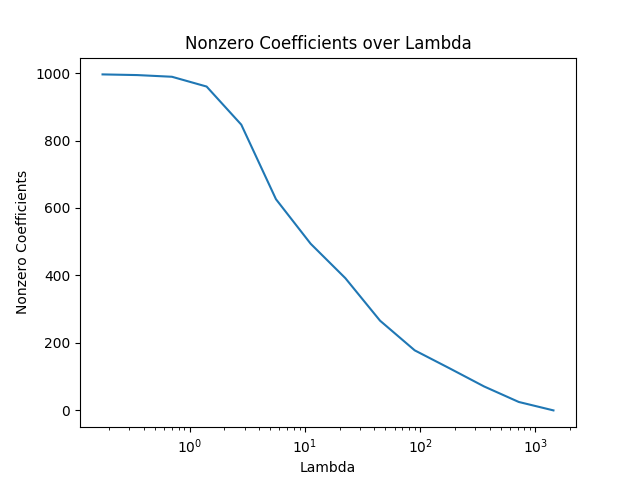
\includegraphics[width=100mm]{../hw2-code/results/a4_a.png}
\end{figure}

\subsection*{b.}

Test accuracy = 96.92\% \\
Test loss = 0.0010

\begin{figure}[h]
  \centering
  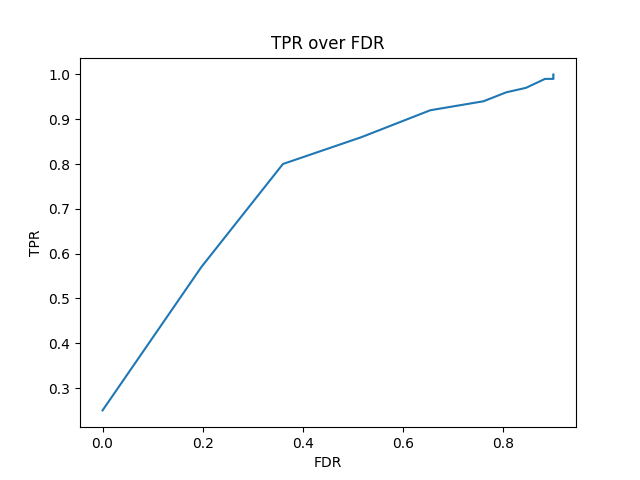
\includegraphics[width=100mm]{../hw2-code/results/a4_b.png}
\end{figure}

\subsection*{c.}

\textbf{Wide and shallow} \\ \\
Number of parameters: $784 \cdot 64 + 64 \cdot 1 + 64 \cdot 10 + 10 \cdot 1 = 50176 + 64 + 640 + 10 = $ \framebox[1.1\width]{\textbf{50890}}  \\
Test accuracy: 97.03\% \\ \\
\textbf{Narrow and deeper} \\ \\
Number of parameters: $784 \cdot 32 + 32 \cdot 1 + 32 \cdot 32 + 32 + 32 \cdot 10 + 10 = 25088 + 32 + 1024 + 32 + 320 + 10 = $ \framebox[1.1\width]{\textbf{26506}} \\
Test accuracy: 96.92\% \\ \\
Although the test accuracies are quite similar in our smaller-scale tests, intuitively, narrow and deeper should be better than wider and shallower. In reality, narrow and deeper networks will be more able to generalize across more data with more layers. Shallower networks work better with less data and on a smaller scale since it can effectively "memorize" on a smaller scale, but not generalize.

\newpage

\begin{verbatim}
# -*- coding: utf-8 -*-
"""cse446_hw3_a4.ipynb

Automatically generated by Colaboratory.

Original file is located at
    https://colab.research.google.com/drive/1_SIbwG3BXMDcx1ZjGFNXcLkcuS4C7G_O
"""

# A4
# Imports

import numpy as np
import matplotlib.pyplot as plt
from mpl_toolkits.mplot3d import Axes3D

import torch
import torch.nn as nn
import torch.nn.functional as F
import torch.optim as optim
import torchvision.datasets as datasets
from torchvision import transforms
from tqdm import tqdm

# Constants

learning_rate = 1E-3

# import MNIST

train_data = datasets.MNIST(root="./data", train=True, download=True, transform=transforms.ToTensor())
test_data = datasets.MNIST(root="./data", train=False, download=True, transform=transforms.ToTensor())

train_loader = torch.utils.data.DataLoader(train_data, batch_size=128, shuffle=True)
test_loader = torch.utils.data.DataLoader(test_data, batch_size=128, shuffle=True)

# Helpers

def initialize_weights(mode, h=64, h_0 = 32, h_1 = 32, m=784, n=10):
  print("Initializing weights for " + mode)
  
  alpha = 1 / np.sqrt(m)
  
  d = m
  k = n
  
  if mode == "a":
    W_0 = nn.init.uniform_(torch.empty(h, d), -alpha, alpha)
    b_0 = nn.init.uniform_(torch.empty(h), -alpha, alpha)
    
    W_1 = nn.init.uniform_(torch.empty(k, h), -alpha, alpha)
    b_1 = nn.init.uniform_(torch.empty(k), -alpha, alpha)
    
    W_0.requires_grad = True
    b_0.requires_grad = True
    W_1.requires_grad = True
    b_1.requires_grad = True
    
    return [W_0, W_1, b_0, b_1]

  if mode == "b":
    W_0 = nn.init.uniform_(torch.empty(h_0, d), -alpha, alpha)    
    b_0 = nn.init.uniform_(torch.empty(h_0), -alpha, alpha)
    
    W_1 = nn.init.uniform_(torch.empty(h_1, h_0), -alpha, alpha)
    b_1 = nn.init.uniform_(torch.empty(h_1), -alpha, alpha)

    W_2 = nn.init.uniform_(torch.empty(k, h_1), -alpha, alpha)
    b_2 = nn.init.uniform_(torch.empty(k), -alpha, alpha)

    W_0.requires_grad = True
    b_0.requires_grad = True
    W_1.requires_grad = True
    b_1.requires_grad = True
    W_2.requires_grad = True
    b_2.requires_grad = True

    return [W_0, W_1, W_2, b_0, b_1, b_2]

def f_1(x, W_0, W_1, b_0, b_1):
  temp = torch.matmul(x, W_0.T) + b_0
  return torch.matmul(F.relu(temp), W_1.T) + b_1

def f_2(x, W_0, W_1, W_2, b_0, b_1, b_2):
  temp1 = F.relu(torch.matmul(x, W_0.T) + b_0)
  temp2 = F.relu(torch.matmul(temp1, W_1.T) + b_1)
  return torch.matmul(temp2, W_2.T) + b_2 

def plot_loss(data, title):
  print("plotting loss")

  epochs = list(range(1, len(data) + 1))

  plt.plot(epochs, data)

  plt.title("loss over time")
  plt.xlabel("epochs")
  plt.ylabel("loss")

  plt.savefig(title)

def train_a(params, learning_rate, h=64, m=784, n=10):
  print("training a")

  W_0, W_1, b_0, b_1 = params[0], params[1], params[2], params[3]  

  optimizer = optim.Adam(params, lr=learning_rate)
  
  loss_data = []
  
  while True:

    acc = 0.
    loss_sum = 0.

    for x, y in tqdm(train_loader):
      x = x.view(-1, m)

      predictions = f_1(x, W_0, W_1, b_0, b_1)

      acc += torch.sum(torch.argmax(predictions, dim=1) == y)

      loss = F.cross_entropy(predictions, y)
      optimizer.zero_grad()
      loss.backward()
      optimizer.step()

      loss_sum += loss
    
    loss_data.append(loss_sum / len(train_loader.dataset))
    acc = acc / len(train_loader.dataset)

    if acc >= 0.99:
      break
  
  return loss_data, [W_0, W_1, b_0, b_1]

def test_a(params):
  print("testing a")

  acc = 0.
  loss_sum = 0.

  W_0, W_1, b_0, b_1 = params[0], params[1], params[2], params[3]

  for x, y in tqdm(test_loader):
    x = torch.flatten(x, start_dim=1, end_dim=3)

    predictions = f_1(x, W_0, W_1, b_0, b_1)

    acc += torch.sum(torch.argmax(predictions, dim=1) == y)
    loss_sum += F.cross_entropy(predictions, y)
  
  acc /= len(test_loader.dataset)
  loss_sum /= len(test_loader.dataset)

  return acc, loss_sum

######################## part (a) ########################

params = initialize_weights("a")
a_train_loss, params = train_a(params, learning_rate)
plot_loss(a_train_loss, "a4_a")

a_test_acc, a_test_loss = test_a(params)
print(a_test_acc)
print(a_test_loss)

def train_b(params, learning_rate, h=32, m=784):
  print("training b")

  W_0, W_1, W_2, b_0, b_1, b_2 = params[0], params[1], params[2], params[3], params[4], params[5]

  optimizer = optim.Adam(params, lr=learning_rate)
    
  acc_data = []
  loss_data = []

  while True:

    acc = 0.
    loss_sum = 0.

    for x, y in tqdm(train_loader):
      x = x.view(-1, m)

      predictions = f_2(x, W_0, W_1, W_2, b_0, b_1, b_2)

      acc += torch.sum(torch.argmax(predictions, dim=1) == y)

      loss = F.cross_entropy(predictions, y)
      optimizer.zero_grad()
      loss.backward()
      optimizer.step()

      loss_sum += loss
    
    loss_data.append(loss_sum / len(train_loader.dataset))
    acc = acc / len(train_loader.dataset)
    
    if acc >= 0.99:
      break
  
  return loss_data, [W_0, W_1, W_2, b_0, b_1, b_2]

def test_b(params):
  print("testing b")

  acc = 0.
  loss_sum = 0.
  
  W_0, W_1, W_2, b_0, b_1, b_2 = params[0], params[1], params[2], params[3], params[4], params[5]
  
  for x, y in tqdm(test_loader):
    x = torch.flatten(x, start_dim=1, end_dim=3)

    predictions = f_2(x, W_0, W_1, W_2, b_0, b_1, b_2)

    acc += torch.sum(torch.argmax(predictions, dim=1) == y)
    loss_sum += F.cross_entropy(predictions, y)
  
  acc /= len(test_loader.dataset)
  loss_sum /= len(test_loader.dataset)

  return acc, loss_sum

######################## part (b) ########################
params = initialize_weights("b")
b_train_loss, params = train_b(params, learning_rate)
plot_loss(b_train_loss, "a4_b")

b_test_acc, b_test_loss = test_b(params)
print(b_test_acc)
print(b_test_loss)

\end{verbatim}

}

\section*{A.5}
{\Large 

\begin{figure}[h]
  \centering
  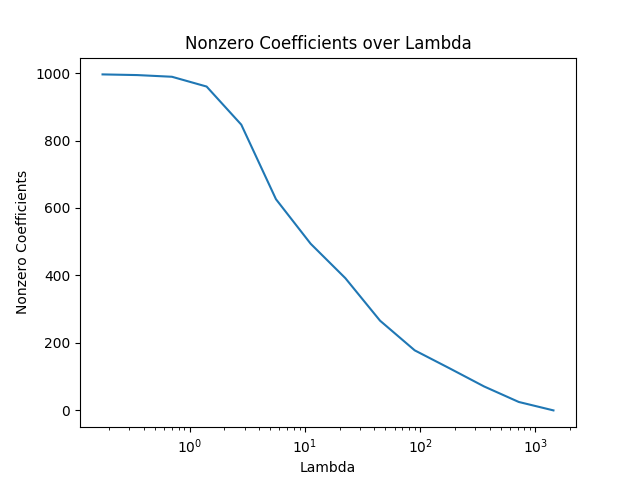
\includegraphics[width=120mm]{../hw2-code/results/a4_a.png}
\end{figure}

\framebox[1.1\width]{\textbf{Applicable output can be found in a5.txt,}} \\
\framebox[1.1\width]{\textbf{which I did not paste in due to its length}}

So far we have trained very small neural networks from scratch. As mentioned in the previous problem, modern neural networks are much larger and more difficult to train and validate. In practice, it is rare to train such large networks from scratch. This is because it is difficult to obtain both the massive datasets and the computational resources required to train such networks. \\
 
 Instead of training a network from scratch, in this problem, we will use a network that has already been trained on a very large dataset (ImageNet) and adjust it for the task at hand. This process of adapting weights in a model trained for another task is known as \textit{transfer learning}.
\begin{itemize}
    \item Begin with the pretrained \text{AlexNet} model from \texttt{torchvision.models} for both tasks below. \text{AlexNet} achieved an early breakthrough performance on \texttt{ImageNet} and was instrumental in sparking the deep learning revolution in 2012.
    \item Do not modify any module within AlexNet that is not the final classifier layer.
    \item The output of AlexNet comes from the $6$-th layer of the classifier. Specifically, \texttt{model.classifer[6] = nn.Linear(4096, 1000)}. To use AlexNet with CIFAR-10, we will reinitialize (replace) this layer with \texttt{nn.Linear(4096, 10)}. This re-initializes the weights, and changes the output shape to reflect the desired number of target classes in CIFAR-10. 
\end{itemize}

\subsection*{a.}

\textbf{Use AlexNet as a fixed feature extractor:} Add a new linear layer to replace the existing classification layer, and only adjust the weights of this new layer (keeping the weights of all other layers fixed). Provide plots for training loss and validation loss over the number of epochs. Report the highest validation accuracy achieved. Finally, evaluate the model on the test data and report both the accuracy and the loss.  
    
    When using AlexNet as a fixed feature extractor, make sure to freeze all of the parameters in the network \textit{before} adding your new linear layer:
    \begin{verbatim}
    model = torchvision.models.alexnet(pretrained=True)
    for param in model.parameters():
        param.requires_grad = False
    model.classifier[6] = nn.Linear(4096, 10)
    \end{verbatim}

\subsection*{b.}

\textbf{Fine-Tuning:} The second approach to transfer learning is to fine-tune the weights of the pre-trained network, in addition to training the new classification layer. In this approach, all network weights are updated at every training iteration; we simply use the existing AlexNet weights as the ``initialization'' for our network (except for the weights in the new classification layer, which will be initialized using whichever method is specified in the constructor) prior to training on CIFAR-10. Following the same procedure, report all the same metrics and plots as in the previous question. 

}

\section*{A.6}
{\Large 

\begin{figure}[h]
  \centering
  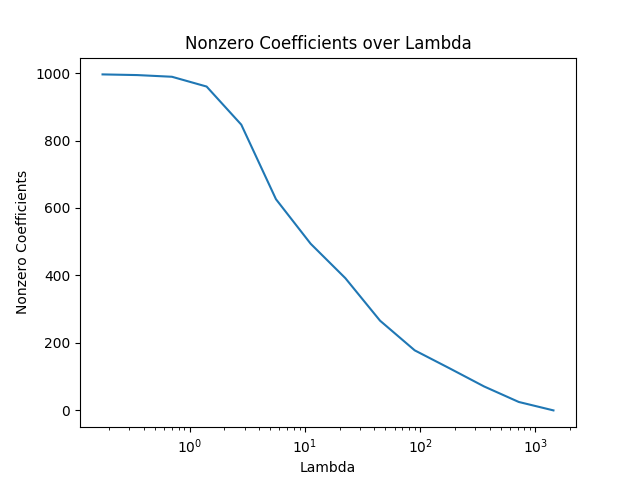
\includegraphics[width=120mm]{../hw2-code/results/a4_a.png}
\end{figure}

\framebox[1.1\width]{\textbf{Applicable output can be found in a6a.txt / a6b.txt / a6c.txt / a6d.txt,}} \\
\framebox[1.1\width]{\textbf{which I did not paste in due to its length}}

\subsection*{a.}

\textbf{Fully-connected output, 0 hidden layers (logistic regression):} this network has no hidden layers and linearly maps the input layer to the output layer. This can be written as 
  \begin{align*}
    x^{\rm out} &= W (x^{\rm in}) +b
  \end{align*} 
  
  where $x^{\rm out} \in \R^{10}$, $x^{\rm in} \in \R^{32 \times 32 \times 3}$, $W \in \R^{10 \times 3072}$, $b \in \R^{10}$ since $3072 = 32 \cdot 32 \cdot 3$. For a tensor $x \in \R^{a \times b \times c}$, we let $(x) \in \R^{a b c}$ be the reshaped form of the tensor into a vector (in an arbitrary but consistent pattern).

\subsection*{b.}

\textbf{Fully-connected output, 1 fully-connected hidden layer:} this network has one hidden layer denoted as $x^{\rm hidden} \in \R^{M}$ where $M$ will be a hyperparameter you choose ($M$ could be in the hundreds). The non-linearity applied to the hidden layer will be the \texttt{relu} ($\mathrm{relu}(x) = \max\{0,x\}$. This network can be written as
  \begin{align*}
    x^{\rm out} &= W_2 \mathrm{relu}(W_1 (x^{\rm in}) +b_1) + b_2
  \end{align*}
  where $W_1 \in \R^{M \times 3072}$, $b_1 \in \R^M$, $W_2 \in \R^{10 \times M}$, $b_2 \in \R^{10}$.

\subsection*{c.}

\textbf{Convolutional layer with max-pool and fully-connected output:} for a convolutional layer $W_1$ with filters of size $k \times k \times 3$, and $M$ filters (reasonable choices are $M=100$, $k=5$), we have that $\mathrm{Conv2d}(x^{\rm in}, W_1) \in \R^{(33-k) \times (33-k) \times M}$.
  
\begin{itemize}
    \item Each convolution will have its own offset applied to each of the output pixels of the convolution; we denote this as $\mathrm{Conv2d}(x^{\rm in}, W) + b_1$ where $b_1$ is parameterized in $\R^M$. Apply a \texttt{relu} activation to the result of the convolutional layer. 
    \item Next, use a max-pool of size $N \times N$ (a reasonable choice is $N=14$ to pool to $2 \times 2$ with $k=5$) we have that $\textrm{MaxPool}( \mathrm{relu}( \mathrm{Conv2d}(x^{\rm in}, W_1)+b_1)) \in \R^{\lfloor\frac{33-k}{N}\rfloor \times \lfloor\frac{33-k}{N}\rfloor \times M}$.
    \item We will then apply a fully-connected layer to the output to get a final network given as
        \begin{align*}
        x^{\rm output} = W_2 (\textrm{MaxPool}( \mathrm{relu}( \mathrm{Conv2d}(x^{\rm input}, W_1)+b_1))) + b_2
        \end{align*}
  where $W_2 \in \R^{10 \times M (\lfloor\frac{33-k}{N}\rfloor)^2}$, $b_2 \in \R^{10}$.
\end{itemize}

The parameters $M,k,N$ (in addition to the step size and momentum) are all hyperparameters, but you can choose a reasonable value. Tuning can be performed (optionally) in the next subproblem.

\subsection*{d.}

\textbf{Tuning:} Return to the original network you were left with at the end of the tutorial \emph{Training a classifier}. Tune the different hyperparameters (number of convolutional filters, filter sizes, dimensionality of the fully-connected layers, stepsize, etc.) and train for a sufficient number of iterations to achieve a \emph{test accuracy} of at least 70\%. Provide the hyperparameter configuration used to achieve this performance.


}

\section*{}
{\Large 
\newpage

\begin{verbatim}
  # helpers.py
# Applicable helpers for HW3

import numpy as np
import matplotlib.pyplot as plt

import constants as c

def generate_data(n):
  print("generating data")

  f_star = lambda x: 4 * np.sin(np.pi * x) * np.cos(6 * np.pi * x ** 2)

  X = np.random.uniform(0, 1, (n, ))
  error = np.random.normal(0, 1, (n, ))
  Y = f_star(X) + error

  return X, Y, f_star

def ylimit_plot(bot, top):
  plt.ylim(bot, top)

def plot_multiple(title, file_name, x, y, data_list, label_list, ylimits=None):
  print("plotting og, true, and fit")

  plt.plot(x, y, "o")
  
  for data_set in data_list:
    plt.plot(c.x_list, data_set)

  if ylimits is not None:
    ylimit_plot(ylimits[0], ylimits[1])

  plt.title(title)
  plt.xlabel("x values")
  plt.ylabel("y values")
  plt.legend(label_list)

  plt.savefig(c.results_path + file_name + c.png_exten)
  plt.close()

def plot_acc(dataset, legends, filename, set_type, epochs=12):
  
  epoch_list = list(range(1, epochs + 1))
  
  for item in dataset:
    plt.plot(epoch_list, item)

  plt.title(set_type + " accuracy over time")
  plt.xlabel("epochs")
  plt.ylabel("accuracy")
  
  plt.legend(legends)

  plt.savefig(filename)
\end{verbatim}

\begin{verbatim}
# constants.py
# Applicable constants for HW3

import numpy as np
import os

home_dir_path = os.path.dirname(os.path.dirname(os.path.abspath(__file__)))

data_path = home_dir_path + '/data/'
results_path = home_dir_path + '/results/'

png_exten = '.png'

hp_list = list(np.linspace(1, 30, 30))
lamb_list = [10 ** -x for x in np.linspace(0, 10, 11)]

pred_labels = ['Data', 'True', 'Predict']
pct_labels = ['Data', 'True', 'Predict', '5%', '95%']
x_list = list(np.linspace(0, 1, 100))

a3b_ylimits = [-5, 5]
num_fold = 10
B = 300
m = 1000
\end{verbatim}
}

\end{document}